\documentclass[a4paper, 11pt]{report}

% %%%
% Camp 100 Long Form Document Preamble
% %%%

% basic document setup
\usepackage{geometry}
\geometry{
a4paper,
total={170mm,257mm},
left=20mm,
top=20mm,
}
\usepackage[skip=0.7em]{parskip} % put in nice paragraph breaksq
\setlength\parindent{0pt} % get rid of the indent
\setcounter{tocdepth}{0} % set toc depth to only show chapters
\setcounter{secnumdepth}{3} % use section numbering for everything up too and including subsubsection

% remove hyphenation at end of line
\tolerance=1
\emergencystretch=\maxdimen
\hyphenpenalty=10000
\hbadness=10000

% document global variables, defined for all documents and used to fill blanks etc
% this comes at the top of the doc as we use these values throughout the entire preamble
% we also set here the language settings for the backpage of the document as it's easier to declare this as a global variable
\newcommand{\documentsetup}[6]{%
    \def\documentTitle{#1}
    \def\documentSubtitle{#2}
    \def\publishDate{#3}
    \def\documentID{#4}
    \def\documentLanguage{#5} % ISO 639 compliant 2 letter language code
    \def\documentStatus{#6}

    \ifthenelse{\equal{#5}{en}}{
        \def\backPageCampInfo{Camp 100, a project by Woodcraft Folk will bring together members of all ages from across the UK to camp together and live by the Woodcraft Folk values for a week in the summer of 2025. The camp celebrates Woodcraft Folk's 100th birthday and will celebrate it's past century while looking forward to the next 100 years.}
        \def\backPageWcfInfo{Woodcraft Folk is a registered charity in England \& Wales (1148195) and in Scotland (SC039791), and a limited company, registered in England \& Wales (8133727). Registered office: Holyoake House, Hanover Street, Manchester M60 0AS}
        \def\backPageCampSocials{Find Camp 100 on the internet}
        \def\backPageWcfSocials{Find Woodcraft Folk online}
    }%
    {}% false
    \ifthenelse{\equal{#5}{fr}}{
        \usepackage[french]{babel}
        \def\backPageCampInfo{Camp-French}
        \def\backPageWcfInfo{Wcf-French}
        \def\backPageCampSocials{fr}
        \def\backPageWcfSocials{fr}
    }%
    {}% false
    \ifthenelse{\equal{#5}{es}}{
        \def\backPageCampInfo{Camp-Spanish}
        \def\backPageWcfInfo{Wcf-Spanish}
        \def\backPageCampSocials{es}
        \def\backPageWcfSocials{es}
    }%
    {}% false
}



% packages for general use
\usepackage[dvipsnames, table]{xcolor}
\usepackage{graphicx}

\usepackage{tikz}
\usetikzlibrary{calc, shapes.callouts}
\usepackage{adjustbox}
\usepackage{fontawesome}
\usepackage{enumitem}
\usepackage{datetime2}
\usepackage{hyperref}
\usepackage{lastpage}
\usepackage{tcolorbox}
\usepackage{ifthen}
\usepackage{multicol}
\usepackage{multirow}
\usepackage{longtable}
\usepackage{ragged2e}
\usepackage{float}


% configure hyperref to do links & PDF metadata
\hypersetup{
    linktoc=none,
    pdfborderstyle={/S/U/W 1},
    colorlinks=false,
    allbordercolors=blue,
    breaklinks=true,
}
% these ones come in a different block as they must be dealt with at the start of the document
\makeatletter
\AtBeginDocument{
  \hypersetup{
    pdftitle={ \documentTitle },
    pdfauthor={Camp 100},
    pdfsubject={ \documentSubtitle },
    pdfcreator={LaTeX}
  }
}
\makeatother
% redefine \href so it uses text color blue to make links more obvious
\let\oldhref\href
\renewcommand{\href}[2]{\oldhref{#1}{\textcolor{blue}{#2}}}

\newcommand{\internallink}[2]{\hyperref[#1]{\textcolor{blue}{#2}}}


%% COLORS
\definecolor{wcf-accent}{HTML}{6d8f41}
\definecolor{c100-red}{HTML}{F04C58}
\definecolor{c100-green}{HTML}{087F5C}
\definecolor{c100-beige}{HTML}{E9E1CA}
\definecolor{c100-orange}{HTML}{EC7E2C}
\definecolor{c100-grey}{HTML}{545454}

% setup setup fonts
% we manually specify to use the `_Light_Oblique' varient of Quicksand for italics as the font doesn't include an italic face by default.
\usepackage{fontspec}
\setmainfont[Ligatures=TeX, ItalicFont=*_Light_Oblique]{Quicksand}
\setsansfont[Ligatures=TeX, ItalicFont=*_Light_Oblique]{Quicksand}

% tables
\renewcommand{\arraystretch}{1.6} % make cells vertically bigger

\newcommand{\tablehead}[1]{\centering\arraybackslash \cellcolor{c100-grey}\leavevmode\color{white}\textbf{#1}} % we try this as it actually allows automatic linebreaks in the headings
% \newcommand{\tablehead}[1]{\multicolumn{1}{c}{\cellcolor{c100-red}\textcolor{white}{\textbf{#1}}}}



% Document Title Page
% adapted from: https://www.reddit.com/r/LaTeX/comments/faij1n/my_first_cover_page_done_in_latex_is_it/
\newcommand{\makedocumenttitlepage}{\begin{titlepage}
    \begin{tikzpicture}[overlay,remember picture]

        % \fill[black!2] (current page.south west) rectangle (current page.north east);
        
        % line 01
        \begin{scope}[transform canvas ={rotate around ={45:($(current page.north west)+(-.5,-6)$)}}]
        \shade[rounded corners=18pt, left color=c100-orange, right color=c100-orange] ($(current page.north west)+(-.5,-6)$) rectangle ++(9,1.5);
        \end{scope}
        
        % line 02
        \begin{scope}[transform canvas ={rotate around ={45:($(current page.north west)+(.5,-10)$)}}]
        \shade[rounded corners=18pt, left color=c100-green ,right color=c100-green] ($(current page.north west)+(0.5,-10)$) rectangle ++(15,1.5);
        \end{scope}
        
        % line 03
        \begin{scope}[transform canvas ={rotate around ={45:($(current page.north)+(-1.5,-3)$)}}]
        \shade[rounded corners=12pt, left color=c100-grey, right color=c100-grey] ($(current page.north)+(-1.5,-3)$) rectangle ++(9,0.8);
        \end{scope}
        
        % line 04
        \begin{scope}[transform canvas ={rotate around ={45:($(current page.north)+(-3,-8)$)}}]
        \shade[rounded corners=28pt, left color=c100-red, right color=c100-red] ($(current page.north)+(-3,-8)$) rectangle ++(15,1.8);
        \end{scope}
        
        % line 05
        \begin{scope}[transform canvas ={rotate around ={45:($(current page.north west)+(4,-15.5)$)}}]
        \shade[rounded corners=25pt, left color=c100-green, right color=c100-green] ($(current page.north west)+(4,-15.5)$) rectangle ++(30,1.8);
        \end{scope}
        
        % line 06
        \begin{scope}[transform canvas ={rotate around ={45:($(current page.north west)+(13,-10)$)}},]
        \shade[rounded corners=22pt, left color=c100-orange,right color=c100-orange] ($(current page.north west)+(13,-10)$) rectangle ++(15,1.5);
        \end{scope}
        
        % line 07
        \begin{scope}[transform canvas ={rotate around ={45:($(current page.north west)+(19,-5.65)$)}},]
        \shade[rounded corners=12pt, left color=c100-grey,right color=c100-grey] ($(current page.north west)+(19,-5.65)$) rectangle ++(15,0.8);
        \end{scope}
        
        % line 08
        \begin{scope}[transform canvas ={rotate around ={45:($(current page.north west)+(18,-8)$)}},]
        \shade[rounded corners=8pt, left color=c100-green,right color=c100-green] ($(current page.north west)+(18,-8)$) rectangle ++(15,0.6);
        \end{scope}
        
        % line 09
        \begin{scope}[transform canvas ={rotate around ={45:($(current page.north west)+(20,-9)$)}}]
        \shade[rounded corners=20pt, left color=c100-red, right color=c100-red] ($(current page.north west)+(20,-9)$) rectangle ++(14,1.2);
        \end{scope}
        
        \node[inner sep=0pt] () at ($(current page.center)+(5,-11)$){
\includegraphics[width=0.45\textwidth]{../global-logo-c100-wide.png}};
        \node[inner sep=0pt] () at ($(current page.center)+(-5,-11)$){
\includegraphics[width=0.45\textwidth]{../global-logo-wcf-wide.png}};
        
        \node[text width=\textwidth,align=center] at ($(current page.center)+(0,-3.5)$) {{\Huge \documentTitle}};
        
        \node[text width=\textwidth,align=center] at ($(current page.center)+(0,-5.5)$) {{\Large{\textit{\documentSubtitle}}} \\[2em] \large \publishDate};
        
        \end{tikzpicture}
\end{titlepage}
}

% Document Back Page
\newcommand{\makedocumentbackpage}{\newpage
  \thispagestyle{empty}
  \begin{tikzpicture}[overlay,remember picture]

      % \fill[black!2] (current page.south west) rectangle (current page.north east);
      
      % line 01
      \begin{scope}[transform canvas ={rotate around ={45:($(current page.north west)+(-.5,-6)$)}}]
      \shade[rounded corners=18pt, left color=c100-orange, right color=c100-orange] ($(current page.north west)+(-.5,-6)$) rectangle ++(9,1.5);
      \end{scope}
      
      % line 02
      \begin{scope}[transform canvas ={rotate around ={45:($(current page.north west)+(.5,-10)$)}}]
      \shade[rounded corners=18pt, left color=c100-green ,right color=c100-green] ($(current page.north west)+(0.5,-10)$) rectangle ++(15,1.5);
      \end{scope}
      
      % line 03
      \begin{scope}[transform canvas ={rotate around ={45:($(current page.north)+(-1.5,-3)$)}}]
      \shade[rounded corners=12pt, left color=c100-grey, right color=c100-grey] ($(current page.north)+(-1.5,-3)$) rectangle ++(9,0.8);
      \end{scope}
      
      % line 04
      \begin{scope}[transform canvas ={rotate around ={45:($(current page.north)+(-3,-8)$)}}]
      \shade[rounded corners=28pt, left color=c100-red, right color=c100-red] ($(current page.north)+(-3,-8)$) rectangle ++(15,1.8);
      \end{scope}
      
      % line 05
      \begin{scope}[transform canvas ={rotate around ={45:($(current page.north west)+(4,-15.5)$)}}]
      \shade[rounded corners=25pt, left color=c100-green, right color=c100-green] ($(current page.north west)+(4,-15.5)$) rectangle ++(30,1.8);
      \end{scope}
      
      % line 06
      \begin{scope}[transform canvas ={rotate around ={45:($(current page.north west)+(13,-10)$)}},]
      \shade[rounded corners=22pt, left color=c100-orange,right color=c100-orange] ($(current page.north west)+(13,-10)$) rectangle ++(15,1.5);
      \end{scope}
      
      % line 07
      \begin{scope}[transform canvas ={rotate around ={45:($(current page.north west)+(19,-5.65)$)}},]
      \shade[rounded corners=12pt, left color=c100-grey,right color=c100-grey] ($(current page.north west)+(19,-5.65)$) rectangle ++(15,0.8);
      \end{scope}
      
      % line 08
      \begin{scope}[transform canvas ={rotate around ={45:($(current page.north west)+(18,-8)$)}},]
      \shade[rounded corners=8pt, left color=c100-green,right color=c100-green] ($(current page.north west)+(18,-8)$) rectangle ++(15,0.6);
      \end{scope}
      
      % line 09
      \begin{scope}[transform canvas ={rotate around ={45:($(current page.north west)+(20,-9)$)}}]
      \shade[rounded corners=20pt, left color=c100-red, right color=c100-red] ($(current page.north west)+(20,-9)$) rectangle ++(14,1.2);
      \end{scope}

    \end{tikzpicture}
      
    % textual boxes at the bottom of the page
    \begin{tikzpicture}[overlay,remember picture]
      % top left box, textual information about C100
      \node[rectangle, anchor=north west,
              rounded corners=18pt,inner sep=11pt,
              fill=c100-green,
              minimum height=11em] () at
              ($(current page.center)+(-9, -3)$)
              {\parbox[t]{0.55\textwidth}{\color{white} \backPageCampInfo}};

      % top right box, social media contact for C100
      \node[rectangle, anchor=north west,
              rounded corners=18pt,inner sep=11pt,
              fill=c100-red,
              minimum height=11em] () at
              ($(current page.center)+(2,-3)$)
              {\parbox[t]{0.35\textwidth}{\color{white} \backPageCampSocials\\[-0.5em] \begin{itemize}[leftmargin=1.5em]
                \setlength\itemsep{0.7em}
                \item[\faInstagram] camp100wcf
                \item[\faFacebook] camp100wcf
                \item[\faLink] camp100.org.uk
              \end{itemize}}};
      
      % bottom left box, WCF charity disclaimer
      \node[rectangle, anchor=north west,
              rounded corners=18pt,inner sep=11pt,
              fill=c100-red,
              minimum height=11em] () at
              ($(current page.center)+(-9,-8)$)
              {\parbox[t]{0.4\textwidth}{\color{white} \backPageWcfInfo}};
      % bottom middle, WCF social media
      \node[rectangle, anchor=north west,
              rounded corners=18pt,inner sep=11pt,
              fill=c100-orange,
              minimum height=11em] () at
              ($(current page.center)+(-0.95,-8)$)
              {\parbox[t]{0.25\textwidth}{\color{white} \backPageWcfSocials\\[-0.5em] \begin{itemize}[leftmargin=1.5em]
                \setlength\itemsep{0.7em}
                \item[\faInstagram] woodcraftfolk
                \item[\faFacebook] woodcraftfolk
                \item[\faLink] woodcraft.org.uk
              \end{itemize}}};
      % bottom right box, WCF logo
      \node[rectangle, anchor=north west,
              rounded corners=18pt,inner sep=11pt,
              fill=c100-green,
              minimum height=11em] () at
              ($(current page.center)+(4.5,-8)$)
              {\parbox[t]{0.2\textwidth}{\color{white} 
\includegraphics[width=0.2\textwidth]{../global-logo-wcf-black.png}}};
      % very bottom line, document information
      \node[rectangle, anchor=north west,
              rounded corners=12pt,inner sep=11pt,
              fill=c100-grey] () at
              ($(current page.center)+(-9,-13)$)
              {\parbox[t]{0.99\textwidth}{\color{white} \footnotesize{\texttt{\documentID}\ (\texttt{\jobname .tex}) compiled at \texttt{\DTMnow}\ with version \texttt{\documentStatus} in language \texttt{\documentLanguage}}}};
    \end{tikzpicture}
  

}

% section titles
% chapter heading adapted from: https://texblog.net/latex-archive/uncategorized/fancy-chapter-tikz/
\usepackage[explicit]{titlesec}

% we only want to deal with chapters if document class is a report; as it'll break in articles otherwise
\makeatletter
\@ifclassloaded{report}{%
    \titlespacing*{\chapter}{0pt}{30pt}{60pt}

    \titleformat{\chapter}
    {\gdef\chapterlabel{}
    \normalfont\sffamily\Huge\bfseries}
    {\gdef\chapterlabel{\thechapter\ | }}{0pt}
    {\begin{tikzpicture}[remember picture,overlay]
        % line 01
        \begin{scope}[transform canvas ={rotate around ={45:($(current page.north west)+(13,-10)$)}},]
        \shade[rounded corners=12pt, left color=c100-grey,right color=c100-grey] ($(current page.north west)+(21,-7)$) rectangle ++(15,0.8);
        \end{scope}
        % line 02
        \begin{scope}[transform canvas ={rotate around ={45:($(current page.north west)+(13,-10)$)}},]
        \shade[rounded corners=20pt, left color=c100-red,right color=c100-red] ($(current page.north west)+(17,-9)$) rectangle ++(15,1.3);
        \end{scope}
        % line 03
        \begin{scope}[transform canvas ={rotate around ={45:($(current page.north west)+(19,-5.65)$)}},]
        \shade[rounded corners=12pt, left color=c100-orange,right color=c100-orange] ($(current page.north west)+(19,-5)$) rectangle ++(15,0.8);
        \end{scope}
        \node[anchor=west,yshift=1.5em, rectangle,
                rounded corners=18pt,inner sep=11pt,
                fill=c100-green] 
                {\parbox[t]{0.6\textwidth}{\color{white}\chapterlabel#1}};
    \end{tikzpicture}
    }
    % redefine \chapter so it uses pagestyle=fancy
    \makeatletter
    \renewcommand\chapter{\if@openright\cleardoublepage\else\clearpage\fi
    \thispagestyle{fancy}%
    \global\@topnum\z@
    \@afterindentfalse
    \secdef\@chapter\@schapter}
    \makeatother
}
\makeatother



\titleformat{\section}
    {\normalfont\LARGE\sffamily\bfseries\color{black}}
    {\tcbox[colback=c100-green, colframe=c100-green, coltext=white, on line, boxsep=0pt, left=4pt, right=4pt, top=4pt, bottom=4pt]{\thesection}}{0.2em}{#1}
\titleformat{\subsection}
    {\normalfont\Large\sffamily\bfseries\color{black}}
    {\tcbox[colback=c100-green, colframe=c100-green, coltext=white, on line, boxsep=0pt, left=4pt, right=4pt, top=4pt, bottom=4pt]{\thesubsection}}{0.2em}{#1}
\titleformat{\subsubsection}
    {\normalfont\large\sffamily\bfseries\color{black}}
    {\tcbox[colback=c100-green, colframe=c100-green, coltext=white, on line, boxsep=0pt, left=4pt, right=4pt, top=4pt, bottom=4pt]{\thesubsubsection}}{0.2em}{#1}




% headers and footers
\usepackage{fancyhdr}


\pagestyle{fancy}
\fancyhf{}
\fancyfoot[L]{\documentTitle}
\fancyfoot[C]{\textbf{\thepage}\ of \pageref*{LastPage}}
\fancyfoot[R]{\publishDate}
\renewcommand{\footrulewidth}{0.4pt}
\renewcommand{\headrulewidth}{0.0pt}
\addtolength{\topmargin}{-1.59999pt}
\setlength{\headheight}{13.59999pt}

% now we do headers and footers for non-release version watermarks
\AtBeginDocument{
    \usepackage{draftwatermark}
    \DraftwatermarkOptions{
        stamp=false,
        text={\documentStatus},
        color=red!30
    }
    \ifthenelse{\equal{\documentStatus}{proof}}{
        \DraftwatermarkOptions{stamp=true}
    }%
    {}% if not set to 1
    \ifthenelse{\equal{\documentStatus}{draft}}{
        \DraftwatermarkOptions{stamp=true}
    }%
    {}% if not set to 1

    
}

% callouts

\usepackage[framemethod=TikZ]{mdframed}
\mdfsetup{skipabove=\topskip,
skipbelow=\topskip,
leftmargin=0cm,
rightmargin=0cm,
linewidth=3pt
}

% Red callout
\mdfdefinestyle{callout-red}{%
linecolor=c100-red!70,
backgroundcolor=c100-red!10,
topline=false,
bottomline=false,
rightline=false,
frametitlebackgroundcolor=c100-red!30,
}
\newenvironment{callout-red}[1]
    {\begin{mdframed}[style=callout-red,frametitle={#1}]
        }
        {
    \end{mdframed}
    }

% Orange callout
\mdfdefinestyle{callout-orange}{%
linecolor=c100-orange!70,
backgroundcolor=c100-orange!10,
topline=false,
bottomline=false,
rightline=false,
frametitlebackgroundcolor=c100-orange!30,
}
\newenvironment{callout-orange}[1]
    {\begin{mdframed}[style=callout-orange,frametitle={#1}]
        }
        {
    \end{mdframed}
    }

% Green callout
\mdfdefinestyle{callout-green}{%
linecolor=c100-green!70,
backgroundcolor=c100-green!10,
topline=false,
bottomline=false,
rightline=false,
frametitlebackgroundcolor=c100-green!30,
}
\newenvironment{callout-green}[1]
    {\begin{mdframed}[style=callout-green,frametitle={#1}]
        }
        {
    \end{mdframed}
    }

% bold callouts - to be used sparingly

\mdfdefinestyle{bold-callout-generic}{
linewidth=0.0em,
fontcolor=white,
roundcorner=0.25em,
font=\bfseries
}
\newenvironment{callout-bold-green}
    {\begin{mdframed}[style=bold-callout-generic, backgroundcolor=c100-green]
        }
        {
    \end{mdframed}
    }
\newenvironment{callout-bold-orange}
    {\begin{mdframed}[style=bold-callout-generic, backgroundcolor=c100-orange]
        }
        {
    \end{mdframed}
    }
\newenvironment{callout-bold-red}
    {\begin{mdframed}[style=bold-callout-generic, backgroundcolor=c100-red]
        }
        {
    \end{mdframed}
    }


% TIKZ
\tikzset{
    c100-speech-callout/.style= {color = white,
                        draw,
                        shape=rectangle callout,
                        fill = c100-green,
                        rounded corners=0.25em,
                        line width = 0.1em,
                        inner xsep = 0.5em,
                        inner ysep = 0.5em,
                        callout relative pointer={(1.25cm,-1cm)},
                        callout pointer width=2cm,
                        font=\bfseries},
    c100-sc-left/.style= {callout relative pointer={(-1.25cm,-1cm)}}
}

% QR Codes
\usepackage{qrcode}
\usepackage{wrapfig}

\newcommand{\insertqrcode}[2]{%
\begin{wrapfigure}{r}{0.35\textwidth}
  \centering
  \begin{mdframed}[linecolor=c100-green, linewidth=0.2em, roundcorner=0.25em, skipabove=0em, skipbelow=0em]
    \begin{center}
      \qrcode[height=0.9\textwidth, nolinks, level=M, version=4]{#1}
      
      {\small \vspace{0.5em} \href{#1}{#2}}
    \end{center}
    
  \end{mdframed}
\end{wrapfigure}
}

\documentsetup{Guide des r\'eservations}{Instructions pour tout ce qui concerne les r\'eservations}{01 July 2024}{booking-handbook}{fr}{draft}

\usepackage{pdfpages}

\begin{document}
\makedocumenttitlepage

\tableofcontents

\chapter{Introduction}
Bienvenu dans ce guide des r\'eservations, afin de comprendre le processus des r\'eservations pour le Camp 100! Nous esp\'erons que ce guide aidera les groupes et les participants qui veulent r\'eserver leur place pour le Camp 100 et que ce soit un guide d\'etaill\'e pour le d\'ebut de votre voyage pour c\'el\'ebrer nos 100 ans.

\section{Syst\`eme de r\'eservation}
Nous utiliserons le syst\`eme de r\'eservation des camps de Woodcraft Folk pour le Camp 100 (c'est une version modifi\'ee et mise \`a jour par rapport \`a celui que nous avons utilis\'e pour Common Ground et le Camp des Venturers 2023). Des informations sur comment acc\'eder au syst\`eme de r\'eservation et comment l'utiliser sont disponibles dans les prochains paragraphes de ce guide.

\section{Support}
Si vous avez besoin d'aide avec le processus de r\'eservation ou si vous avez des questions qui ne figurent pas dans ce guide, veuillez contacter info@camp100.org.uk 

\section{Aperçu du processus de r\'eservation}
Le processus de r\'eservation a plusieurs parties.
\begin{enumerate}
    \item Demande de r\'eservation \internallink{chap:apply}{(\'etape \ref*{chap:apply})}
    \item R\'eserver \internallink{chap:booking}{(\'etape \ref*{chap:booking})}
    \item Modifier une r\'eservation \internallink{chap:edit}{(\'etape \ref*{chap:edit})}
\end{enumerate}

\section{R\'eservations individuelles}
Si possible, vous devez r\'eserver en tant que groupe. Si vous \^etes une personne qui souhaite camper avec un groupe auquel vous \^etes affili\'e, veuillez contacter votre groupe afin d'\^etre inclus dans leur r\'eservation. 
Si vous souhaitez r\'eserver individuellement en tant que volontaire, veuillez vous r\'ef\'erer \`a la section 2 `comment s\'electionner une r\'eservation individuelle'. Il est possible pour les personnes individuelles (et pour les groupes jusqu'\`a 3 personnes) de payer par carte.


\section{Adh\'erents \`a Woodcraft Folk Membership \& DBS}
Toutes les personnes \^ag\'ees de 16 ans qui participent au camp depuis l'Angleterre doit \^etre adh\'erent de Woodcraft Folk. Les informations sur comment devenir adh\'erent se trouvent sur le site de Woodcrat Folk \href{https://woodcraft.org.uk/get-involved/volunteering-with-woodcraft-folk/}{ici}.

Les adh\'erents de Woodcraft Folk de plus de 16 ans qui ont une mission dans laquelle ils sont responsables de jeune de moins de 16 ans et toutes les personnes de plus de 18 ans doit avoir un DBS / PVG valide. 
Des informations sur comment s'y prendre seront disponibles par votre secr\'etaire aux adh\'esions ou sur \href{https://woodcraft.org.uk/get-involved/volunteering-with-woodcraft-folk/}{le site de Woodcraft Folk}.

Plus d'informations sur la protection au Camp 100 seront disponibles sur notre site d\'edi\'e \`a la protection. 

\section{Protection internationale}
Les campeurs internationaux \^ag\'es de plus de 18 ans doivent signer une d\'eclaration de protection avant de venir au Camp 100. Afin d'assurer la protection et la s\'ecurit\'e de tous les campeurs et volontaires pendant c \'ev\'enement. Les campeurs internationaux \^ag\'es entre 16 et 18 ans qui sont volontaires pendant le camp devront \'egalement signer cette d\'eclaration. Une fois votre r\'eservation effectu\'ee vous recevrez une copie \'electronique de la d\'eclaration \`a signer sur l'adresse email fournie. 



\chapter{Etape 1: Demande de r\'eservation}
\label{chap:apply}
La 1re \'etape pour la r\'eservation est de faire une demande. Vous devez faire cette demande pour cr\'eer une r\'eservation. Faire une demande de r\'eservation n'est pas un engagement, cela est juste \`a titre indicatif pour nous donner une id\'ee du nombre de participants. Les groupes venant hors d'Europe de l'Ouest doivent faire cette demande avant le 1re d\'ecembre 2024 afin que nous puissions candidater \`a des financements (cependant nous ne pourrons pas financer tous les groupes qui le demandent). Une fois votre demande valid\'ee, vous pourrez vous connecter et modifier votre r\'eservation. 

\begin{enumerate}
    \item Rendez vous sur \href{https://bookings.camp100.org.uk}{Camp 100 syst\`eme de r\'eservation}
    \item Cliquez sur vous connecter pour r\'eserver.\\
    A côt\'e du bouton de connexion se trouve un bouton pour activer le mode sombre/clair. Cela va vous permettre de changer le th\`eme du site en mode sombre ou clair. Pour des raisons de simplicit\'e, toutes les captures d'\'ecran dans ce guide seront en mode clair. 
    \begin{figure}[H]
        \centering
        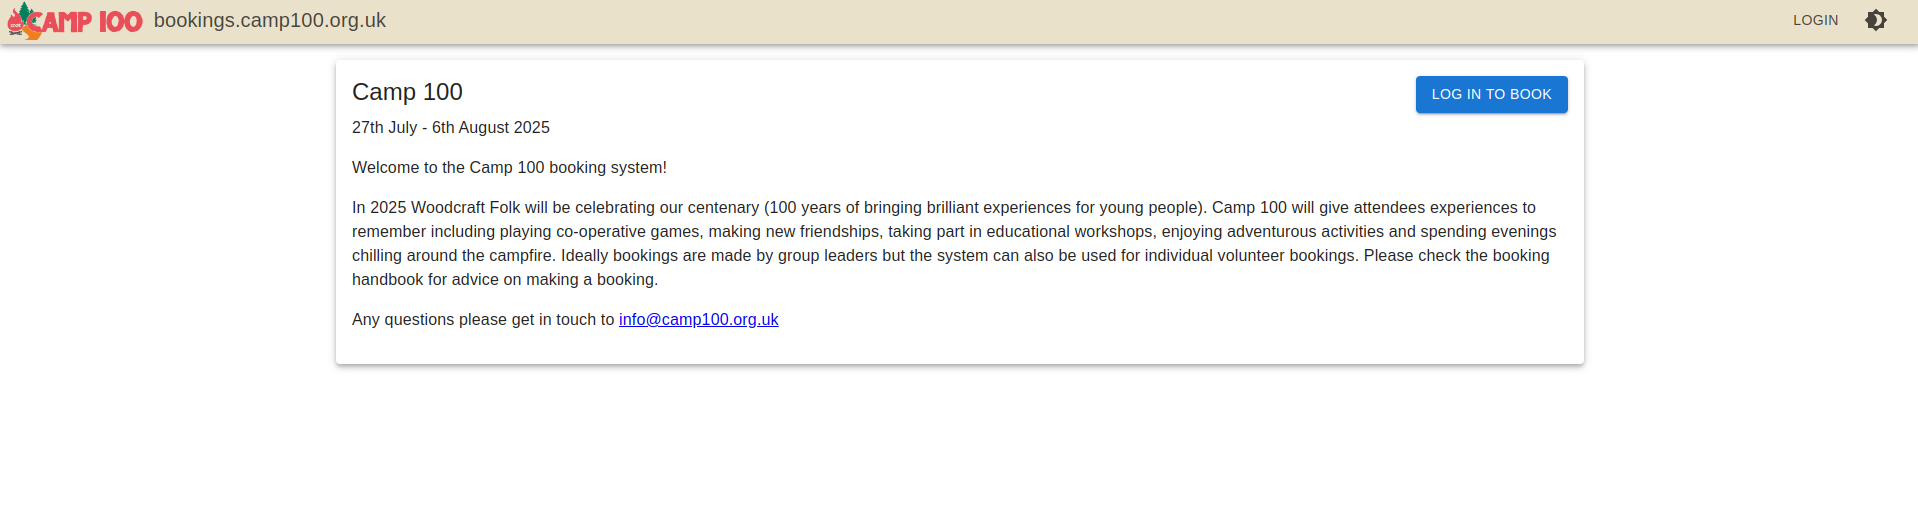
\includegraphics[width=0.9\textwidth]{assets/1-homepage.png}
        \caption{Page d'accueil du syst\`eme de r\'eservation}
    \end{figure}
    \item S\'electionnez une des mani\`eres de connexion
    \begin{figure}[H]
        \centering
        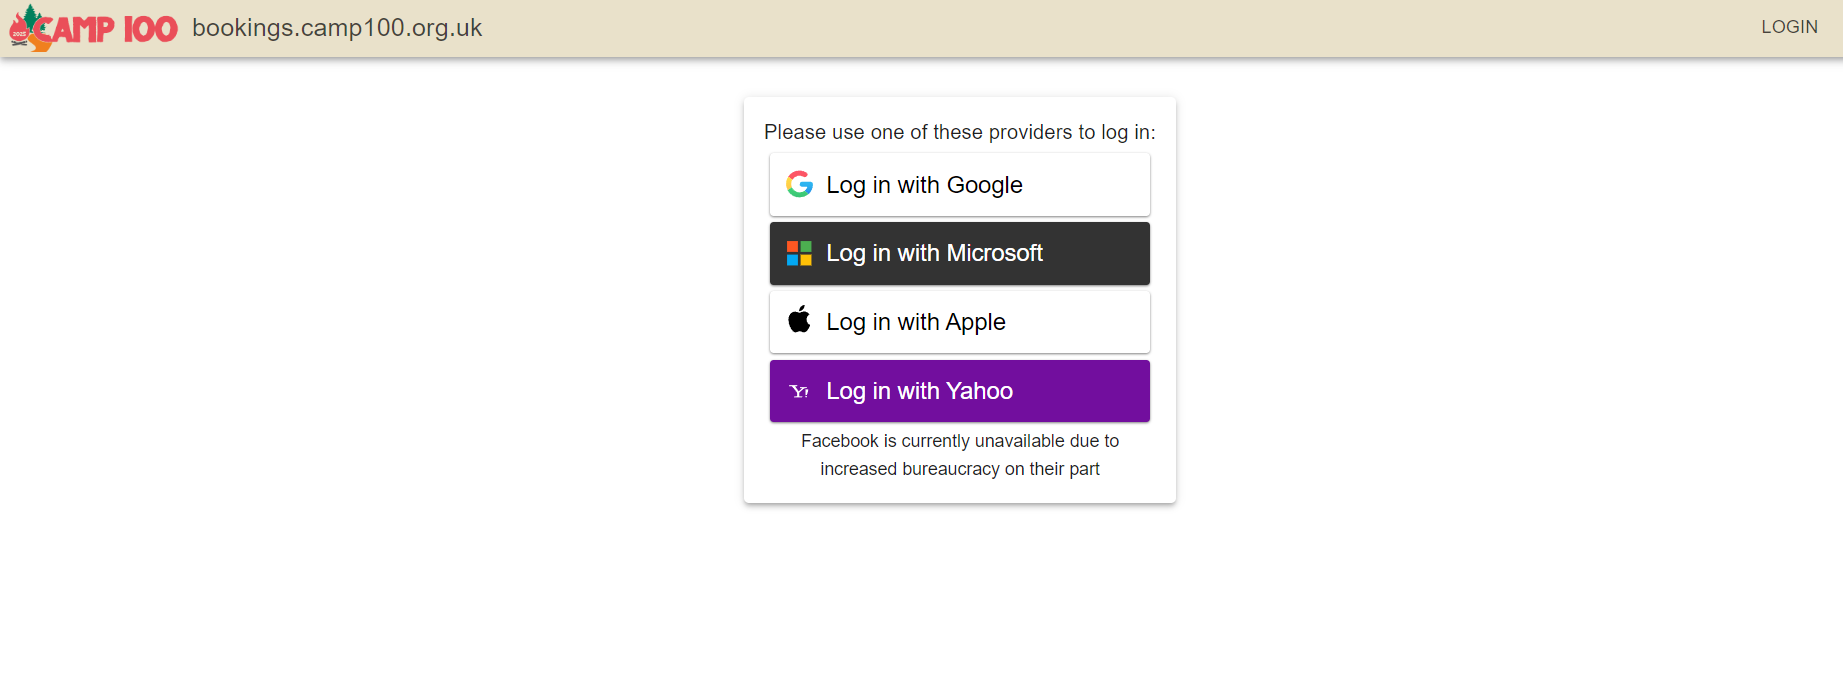
\includegraphics[width=0.9\textwidth]{assets/1-login.png}
        \caption{Options de connexion}
    \end{figure}
    \item Suivez les instructions sur l'\'ecran.
    \item Une fois que vous vous \^etes connect\'e, vous serez redirig\'e vers l'\'ecran du dessous. Votre nom apparaîtra dans le coin en haut \`a droite. Entrez votre nom et rentez votre adresse mail, puis cliquez sur enregistrer.
    \begin{figure}[H]
        \centering
        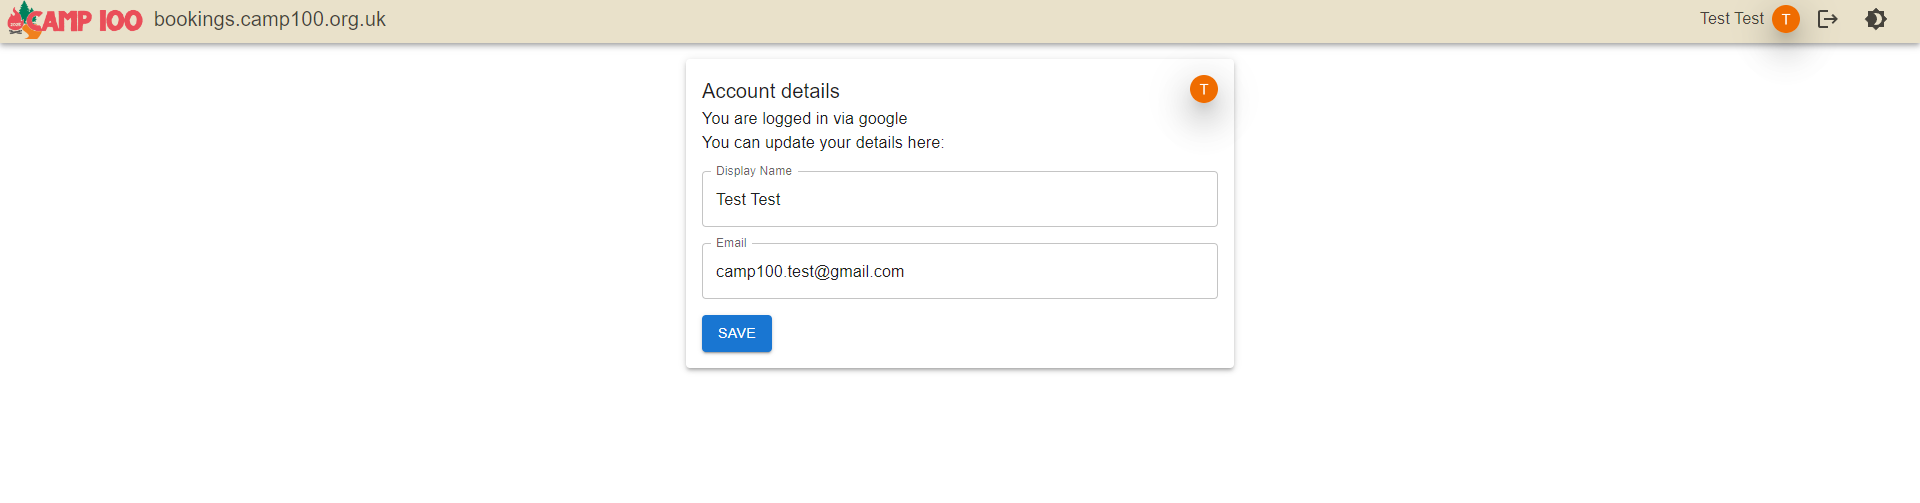
\includegraphics[width=0.9\textwidth]{assets/1-create-account.png}
        \caption{Options de cr\'eation de compte}
    \end{figure}
    \item Vous serez redirig\'e vers la page d'accueil. Cliquez sur `faire une demande' / `Apply to book'
    \begin{figure}[H]
        \centering
        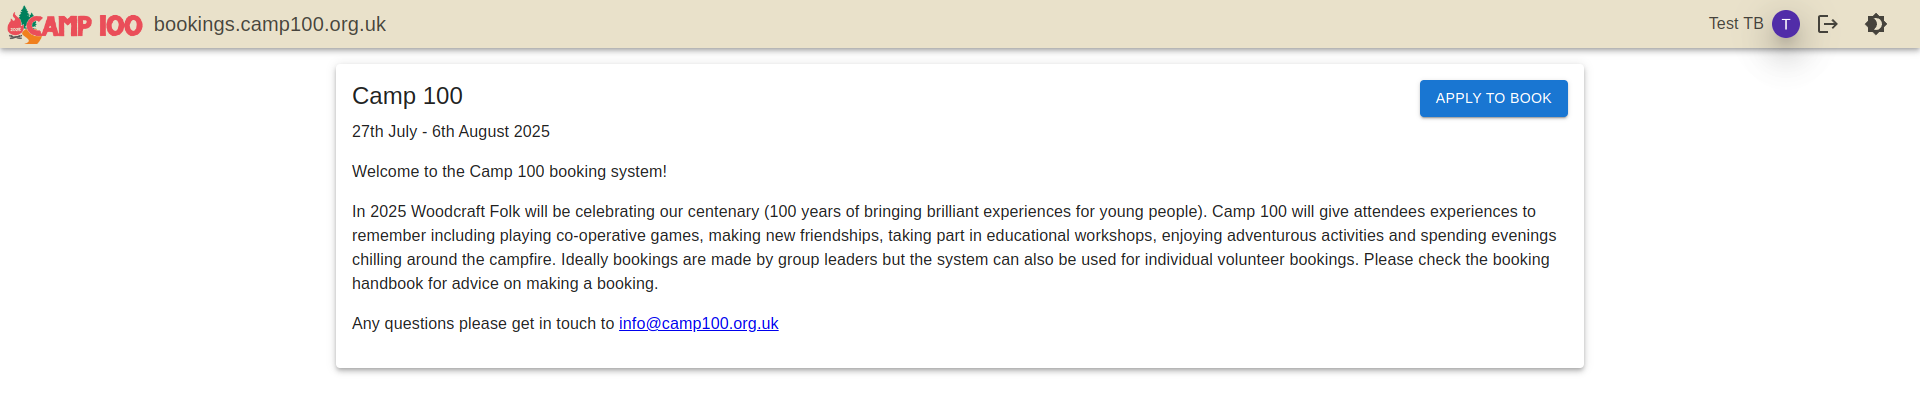
\includegraphics[width=0.9\textwidth]{assets/1-homepage-loggedin.png}
        \caption{Bouton Appliquer au livre}
    \end{figure}
    \item S\'electionnez si vous faites une r\'eservation pour un groupe ou individuelle. Vous devrez rentrer votre nom et votre adresse mail. S\'electionnez votre organisation depuis le menu d\'eroulant et entre un nombre approximatif de participants dans la partie texte, puis cliquez sur `submit'. (Ce n'est pas grave si cela change, une estimation est d\'ej\`a tr\`es utile pour nous.)
    \begin{figure}[H]
        \centering
        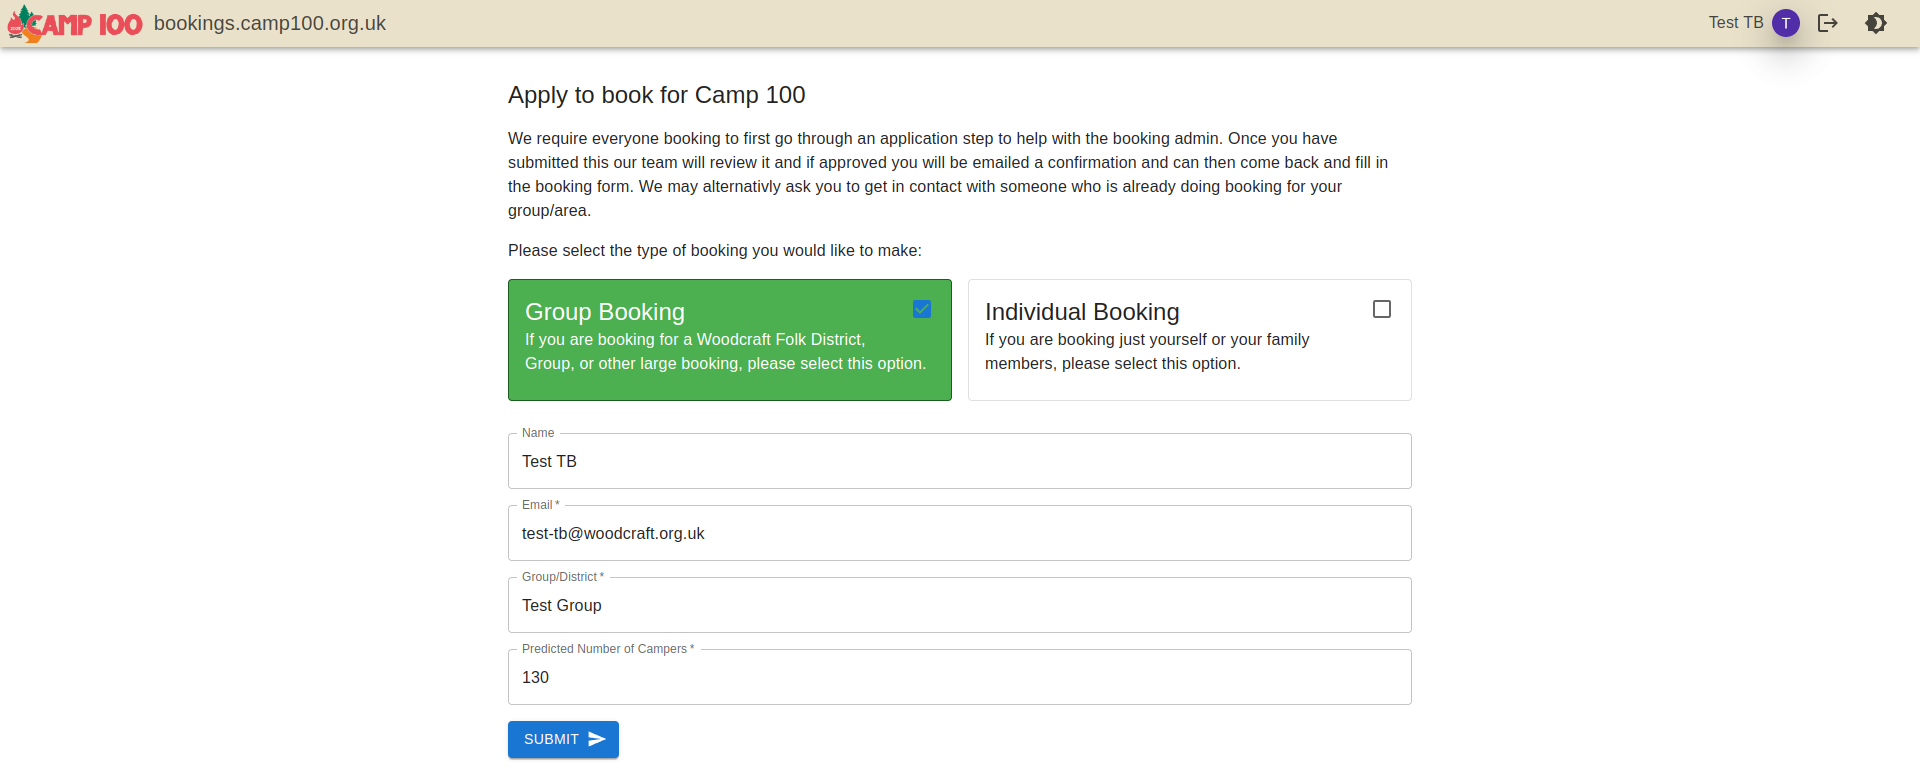
\includegraphics[width=0.9\textwidth]{assets/1-apply.png}
        \caption{Page Postuler au livre}
    \end{figure}
    \item Votre demande sera ensuite envoy\'ee \`a l'\'equipe du Camp 100.
    \item Une fois votre r\'eservation approuv\'ee, vous recevrez un autre e-mail. Continuez jusqu'\`a \internallink{chap:booking}{\'etape 2: R\'eservation}. Si, d'apr\`es votre candidature, il semble qu'une autre personne du m\^eme groupe a d\'ej\`a postul\'e pour r\'eserver, nous pouvons vous contacter pour vous dire que vous devriez lui parler plutôt que de vous autoriser \`a r\'eserver s\'epar\'ement.
\end{enumerate}



\chapter{Etape 2: R\'eserver}
\label{chap:booking}

Pour commencer cette \'etape, votre demande doit \^etre approuv\'ee. Veuillez vous r\'ef\'erer \`a \internallink{chap:apply}{l'\'etape 1: Faire une demande de r\'eservation}.

Le syst\`eme de r\'eservation est fait pour \^etre un syst\`eme en direct. Afin de simplifier au maximum la t\^ache des r\'ef\'erents, nous vous encourageons \`a ajouter les personnes le plus vite possible (m\^eme si le processus de r\'eservation de votre groupe est toujours en cours), afin de le faire au fil de l'eau et donner une estimation \`a l'\'equipe du Camp 100.

\begin{enumerate}
    \item Rendez vous sur \href{https://bookings.camp100.org.uk}{Camp 100 syst\`eme de r\'eservation}
    \item Cliquez `se connecter pour r\'eserver' / `login to book' et utilisez le m\^eme service que la derni\`ere fois (cela est tr\`es important sinon vous ne pourrez pas vous connecter).
    \begin{figure}[H]
        \centering
        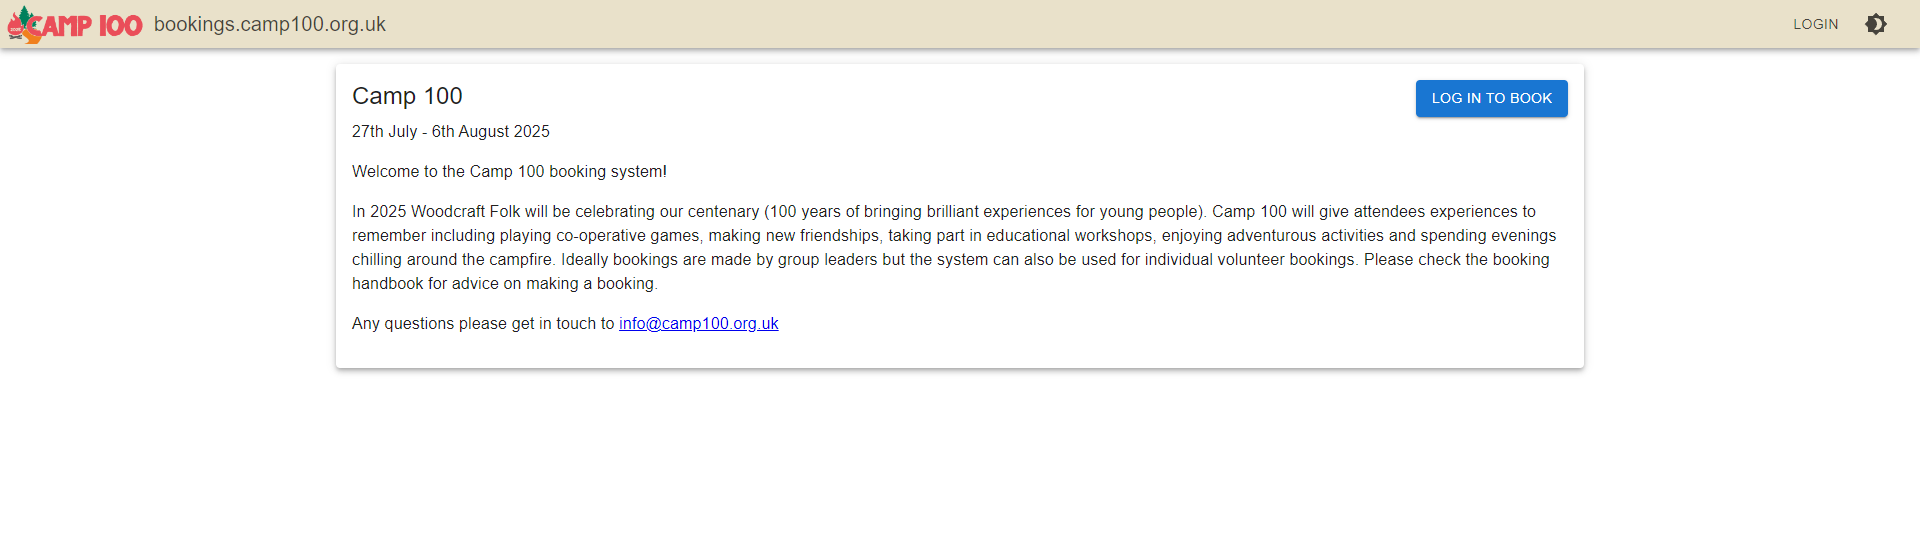
\includegraphics[width=0.9\textwidth]{assets/2-home-prelogin.png}
        \caption{Page d'accueil du syst\`eme de r\'eservation}
    \end{figure}
    \item Vous serez redirig\'e vers la page d'acceuil. Cliquez sur R\'eserver.
    \begin{figure}[H]
        \centering
        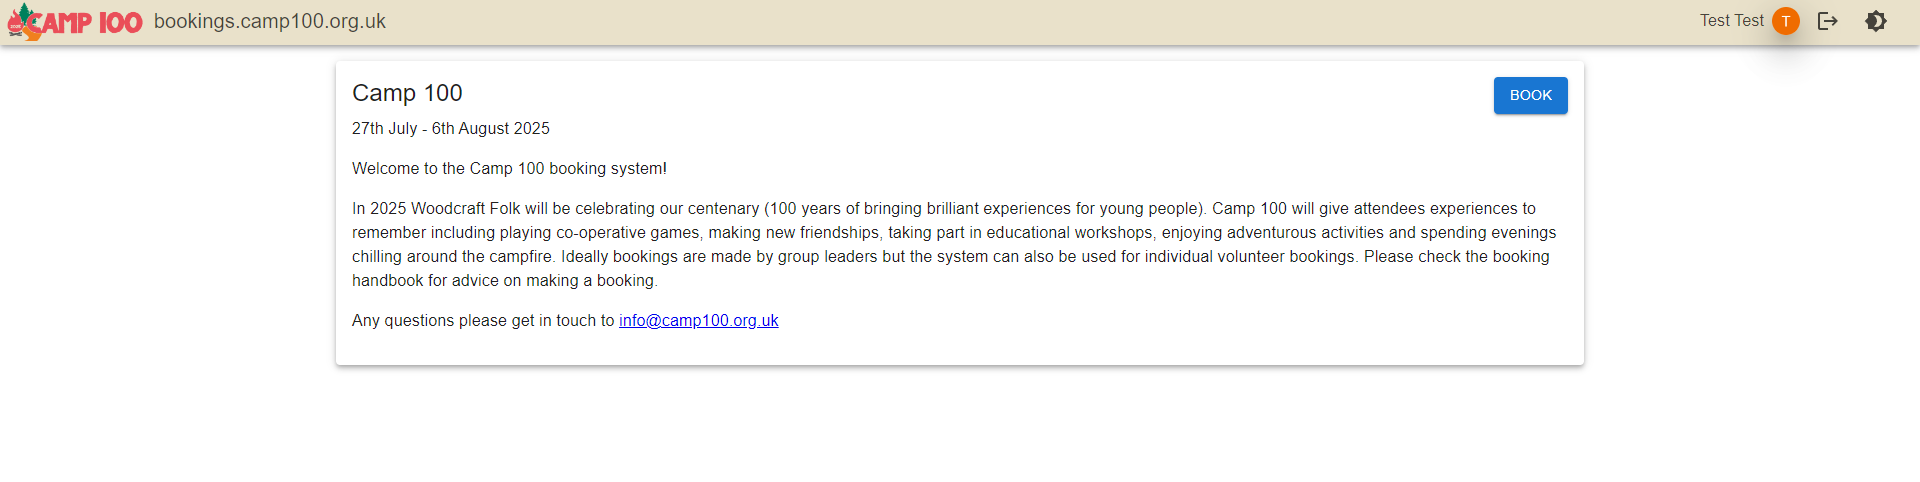
\includegraphics[width=0.9\textwidth]{assets/2-home-loggedin.png}
        \caption{Page d'accueil affichant le bouton `R\'eserver'}
    \end{figure}
    \item Maintenant, nous devez renseigner des informations sur votre r\'eservation. Entrez ces informations dans les parties de textes. Vous avez la possibilit\'e d'ajouter `des contacts en plus', ce sont vos volontaires qui font partie de votre r\'eservation et que l'\'equipe du Cap 100 peut contacter. 
    \item Descendez jusqu'\`a `Campers' / `Campeurs'
    \item Nous avons ajout\'e une option pour compl\'eter le formulaire de r\'eservation dans un tableau excel plutôt qu'utiliser un formulaire individuel dans le syst\`eme pour chaque campeur. Vous devez choisir si vous voulez rentrer les informations dans un tableau excel  \textbf{OU} compl\'eter la r\'eservation en utilisant les formulaires dans le syst\`eme de r\'eservation. 
    
    Si vous n'utilisez \textbf{PAS} l'option du tableau excel, rendez-vous \internallink{manual-import}{au paragraphe \ref*{manual-import}}

    Consignes pour le tableau excel: 
    \begin{enumerate}
        \item Nous pouvons cr\'eer un Google Sheet pour remplir et importer les informations. Cela peut \^etre utile pour les grands groupes. Cliquez sur le bouton `cr\'eer un Google Sheet' va cr\'eer un Google Sheet avec l'adresse mail que vous avez fourni. Les m\^emes informations seront demand\'ees dans le tableau excel que dans le syst\`eme de r\'eservation.
        
        \textbf{NOTE: importer les informations dans le tableau excel effacera les informations que vous avez entr\'ees dans le formulaire donc c'est important que vous choisissiez quelle m\'ethode vous utilisez.}
        \begin{figure}[H]
            \centering
            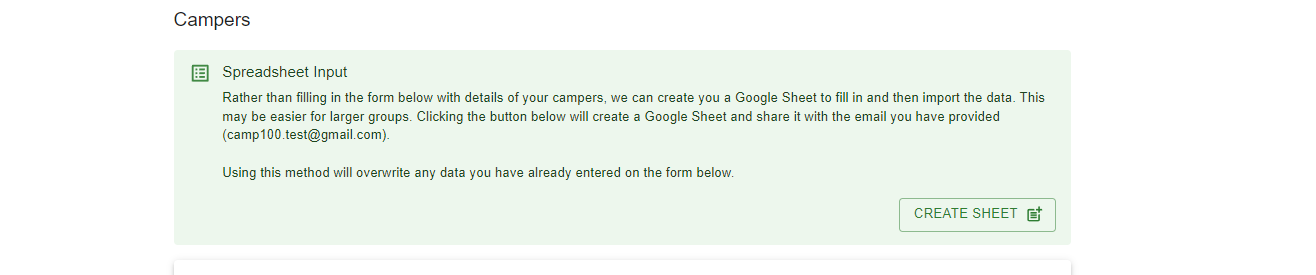
\includegraphics[width=0.9\textwidth]{assets/2-spreadsheet-option.png}
            \caption{Bouton Cr\'eer une feuille}
        \end{figure}
        \item Une fois que vous cr\'eez votre tableau excel vous recevrez un email avec un lien. Pour acc\'eder au tableau excel vous devez avoir un compte google (vous pouvez cr\'eer un compte google avec une adresse gmail, veuillez vous r\'ef\'erer \`a cet article - \href{https://support.google.com/accounts/answer/27441?hl=fr}{support.google.com/accounts/answer/27441} ) 
        \item Une fois que vous avez reçu l'email vous pouvez suivre le lien pour ouvrir le document.
         \begin{figure}[H]
            \centering
            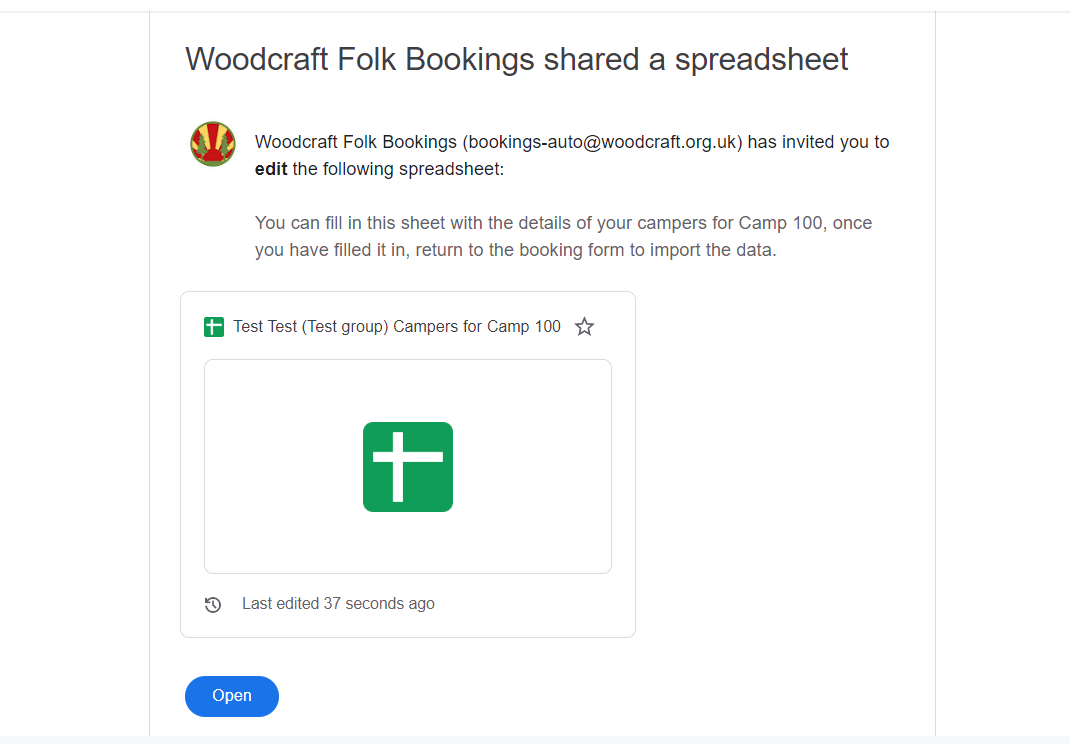
\includegraphics[width=0.6\textwidth]{assets/2-spreadsheet-email.png}
            \caption{E-mail montrant la feuille de calcul partag\'ee}
        \end{figure}
        \item Une fois que vous avez ouvert le document, vous verrez les m\^emes champs \`a remplir que dans le formulaire de r\'eservation. Nous vous conseillons de partager  \internallink{chap:template-booking-form}{l'exemple du formulaire de consentement} qui se trouve \`a la fin de ce guide aux parents et responsables de votre groupe et d'utiliser les informations de chaque campeur pour remplir le tableau. Nous avons besoin d'une adresse mail pour chaque campeur, si le campeur est \^ag\'e de moins de 16 ans, c'est l'adresse mail de son parent ou responsable l\'egal qui doit \^etre renseign\'ee. Nous utiliserons cette adresse mail pour informer les campeurs/parents ou responsables et v\'erifier leur adh\'esion \`a Woodcraft Folk.
        \begin{figure}[H]
            \centering
            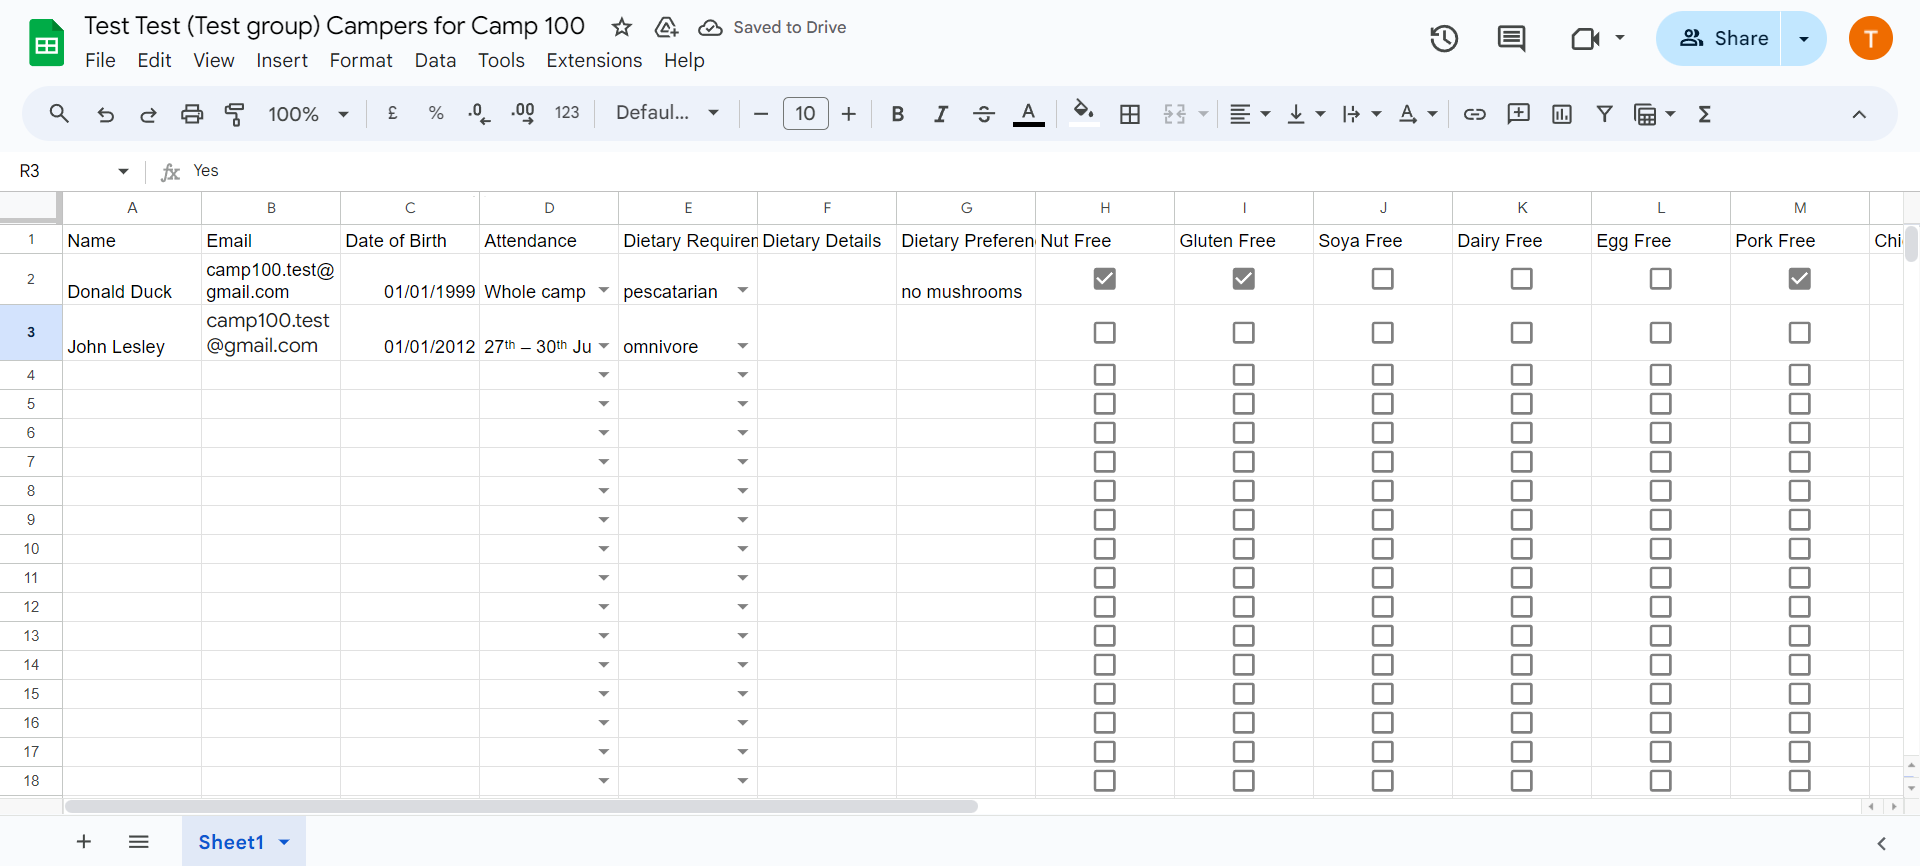
\includegraphics[width=0.9\textwidth]{assets/2-spreadsheet.png}
            \caption{Feuille de calcul montrant des exemples d'informations sur les campeurs}
        \end{figure}
        \item Vous pouvez revenir sur le tableau et le mettre \`a jour, ajouter des nouveaux participants et en enlever \`a tout moment, avant la date de fin, l'enregistrement se fera automatiquement dans le Google Sheet. Vous pouvez importer les informations dans le syst\`eme de r\'eservation \`a n'importe quel moment en revenant dans le syst\`eme de r\'eservation et en cliquant sur `importer les donn\'ees'  \textbf{NOTE: importer depuis le tableau excel effacera les donn\'ees que vous avez entr\'ees dans le formulaire du syst\`eme de r\'eservation.}
        \begin{figure}[H]
            \centering
            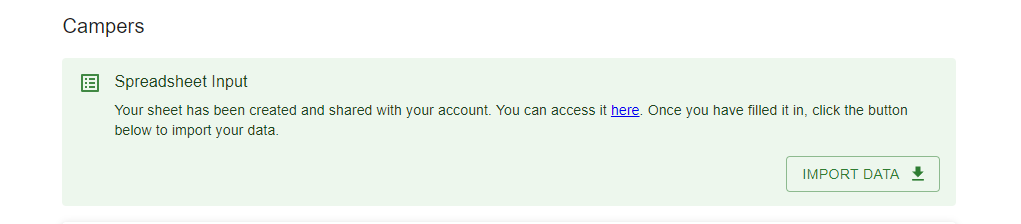
\includegraphics[width=0.9\textwidth]{assets/2-spreadsheet-import.png}
            \caption{Bouton `Importer des donn\'ees'}
        \end{figure}
        \item Une fois que vos donn\'ees ont \'et\'e import\'ees, les informations du campeur seront retranscrites dans le champ du formulaire du syst\`eme de r\'eservation. Les participants seront list\'es dans la partie droite de l'\'ecran, ce qui vous permettra de v\'erifier le nombre total de participants.
        \begin{figure}[H]
            \centering
            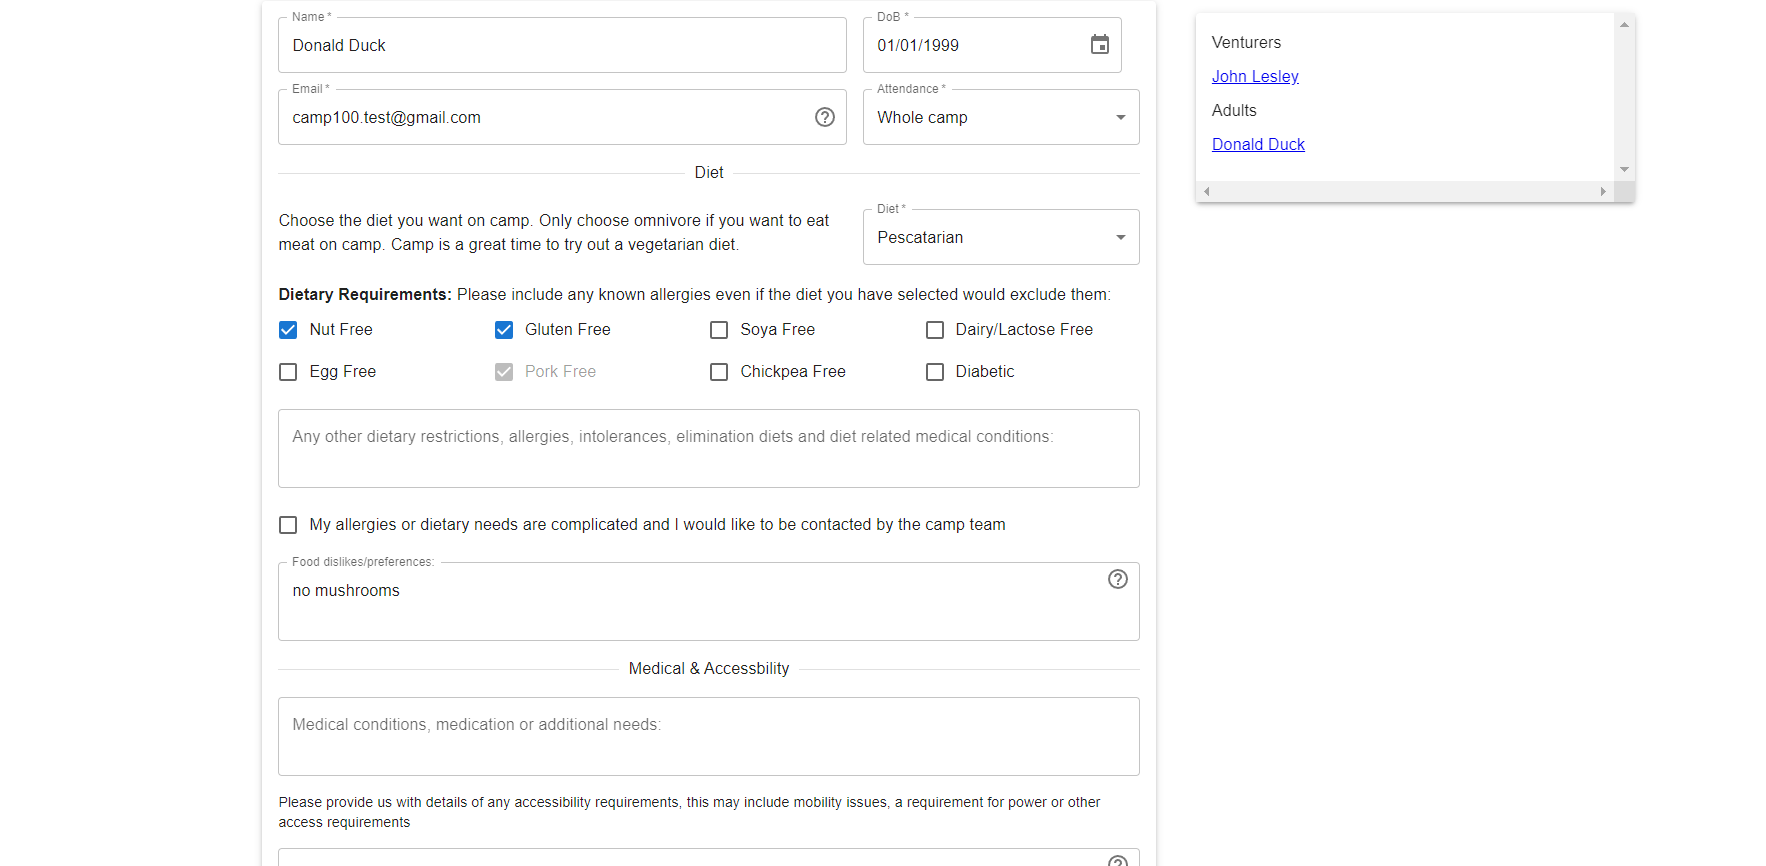
\includegraphics[width=0.9\textwidth]{assets/2-spreadsheet-review.png}
            \caption{Les donn\'ees import\'ees de la feuille de calcul s'affichent sur le syst\`eme de r\'eservation}
        \end{figure}
        \item Une fois que vous avez import\'e les informations depuis le tableau vous devez finir de remplir le formulaire et l'envoyer, \internallink{everyone-steps}{rendez-vous \`a la partie \ref*{everyone-steps}} pour compl\'eter votre r\'eservation.
    \end{enumerate}
    \item \label{manual-import}  Si vous n'utilisez pas le tableau excel, vous devez remplir le formulaire ci-dessous pour chacun des participants. Une fois ajout\'es, les campeurs seront affich\'es sur la partie droite de l'\'ecran, ce qui vous permettra de voir le nombre total de participants. Nous avons besoin d'une adresse mail pour chaque participant, si le campeur a moins de 16 ans, veuillez renseigner l'adresse mail d'un parent ou responsable l\'egal. Nous utiliserons les adresses mails pour informer les campeurs/ parents/ responsables et v\'erifier leur adh\'esion \`a Woodcraft Folk.
    \begin{figure}[H]
        \centering
        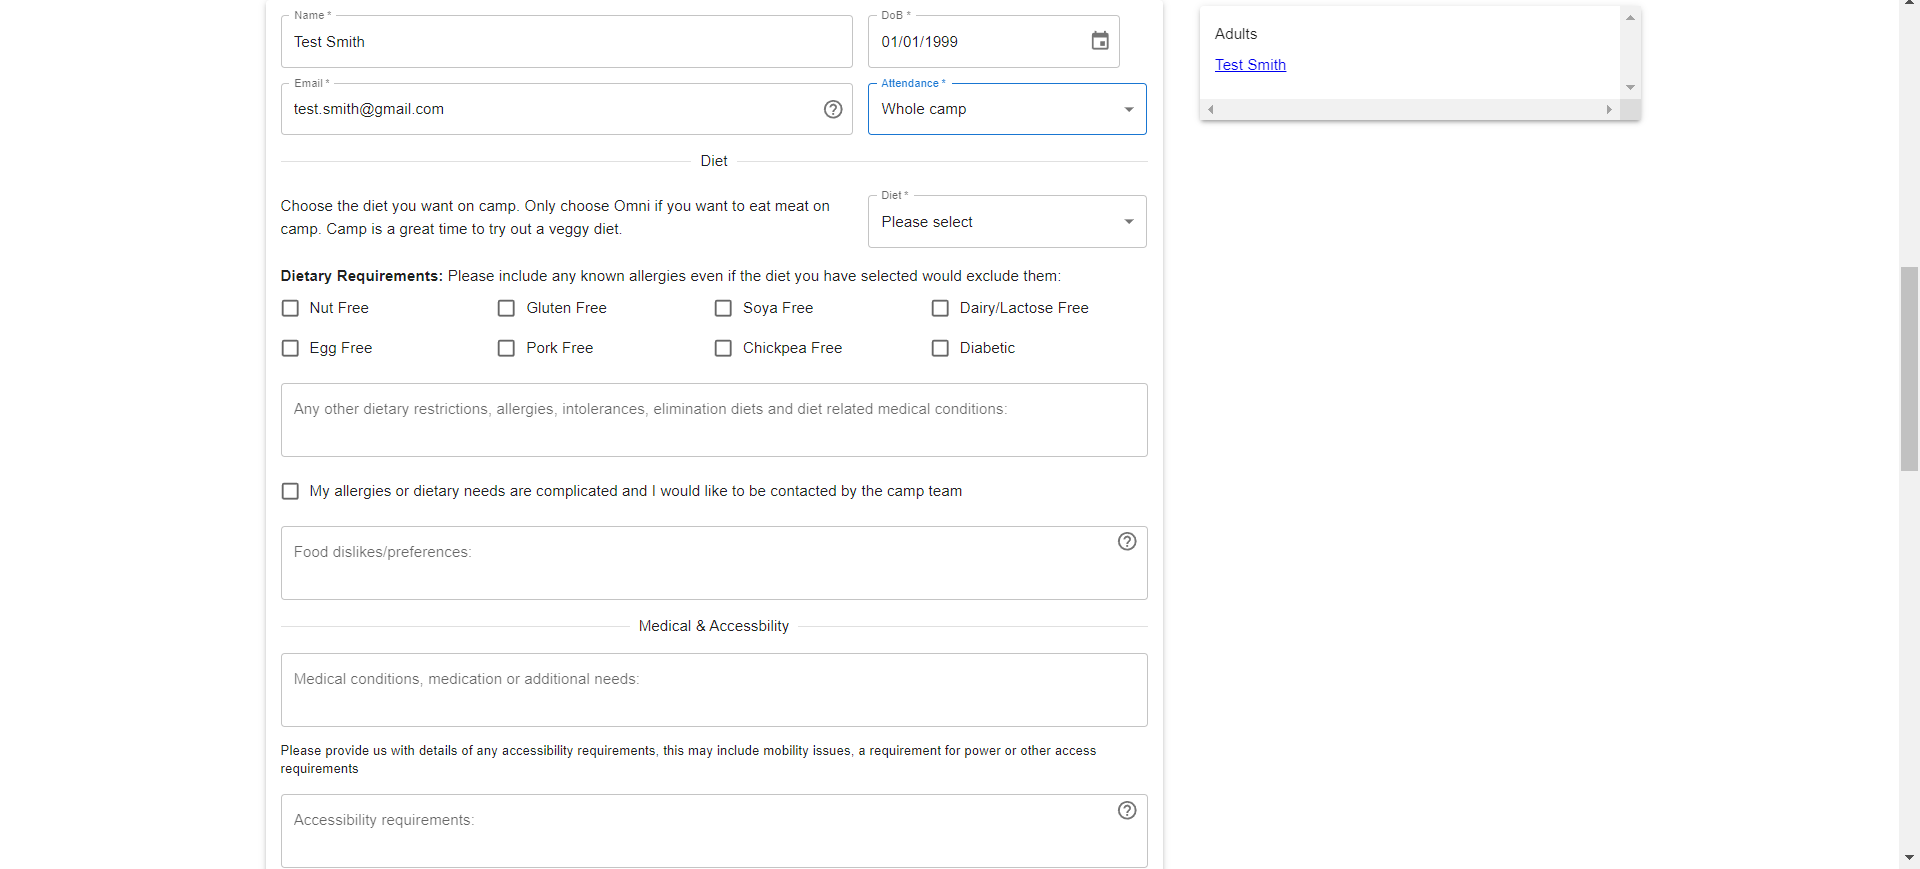
\includegraphics[width=0.9\textwidth]{assets/2-manual-input.png}
        \caption{Saisir manuellement un participant}
    \end{figure}
    \item Pour ajouter plus de campeur, cliquez sur `ajouter une personne' / `add person'. Cela rajoutera un nouveau formulaire vierge \`a remplir.
    \item  Pour enlever un campeur, cliquez sur le bouton orange pour `d\'everrouiller' le bouton supprimer, cliquez sur la croix \`a côt\'e du participant.
    \begin{figure}[H]
        \centering
        
\includegraphics[width=0.9\textwidth]{assets/2-add-person-button.png}
        \caption{Bouton `Ajouter une personne' et cadenas orange}
    \end{figure}
    \item \label{everyone-steps}Une fois que vous avez rempli toutes les informations de tous vos participants, descendez en bas de la page jusqu'\`a `camping'. Ici veuillez entrer les informations \`a propos des groupes avec lesquels vous souhaitez camper, le mat\'eriel que vous avez et tous les d\'etails sur les besoins de vos campeurs. Cela peut inclure les besoins des campeurs qui ne sont pas encore renseign\'es. 
    \item  Descendez jusqu'\`a “Argent”/”Money”. Ici, vous aurez une estimation du prix de votre groupe pour participer au camp, votre r\'ef\'erence de paiement C100-XXXXX (devra \^etre utilis\'e pour tous les paiements) et des consignes pour le paiement. Si votre groupe fait la demande d'acc\`es \`a des financements, nous vous informons par email si cela est possible et nous changerons le montant sur le syst\`eme. Veuillez voir la section 3 pour plus d'informations sur le paiement. Voir la \internallink{chap:payment}{Section \ref*{chap:payment}} pour plus d'informations sur le paiement. 
    \begin{figure}[H]
        \centering
        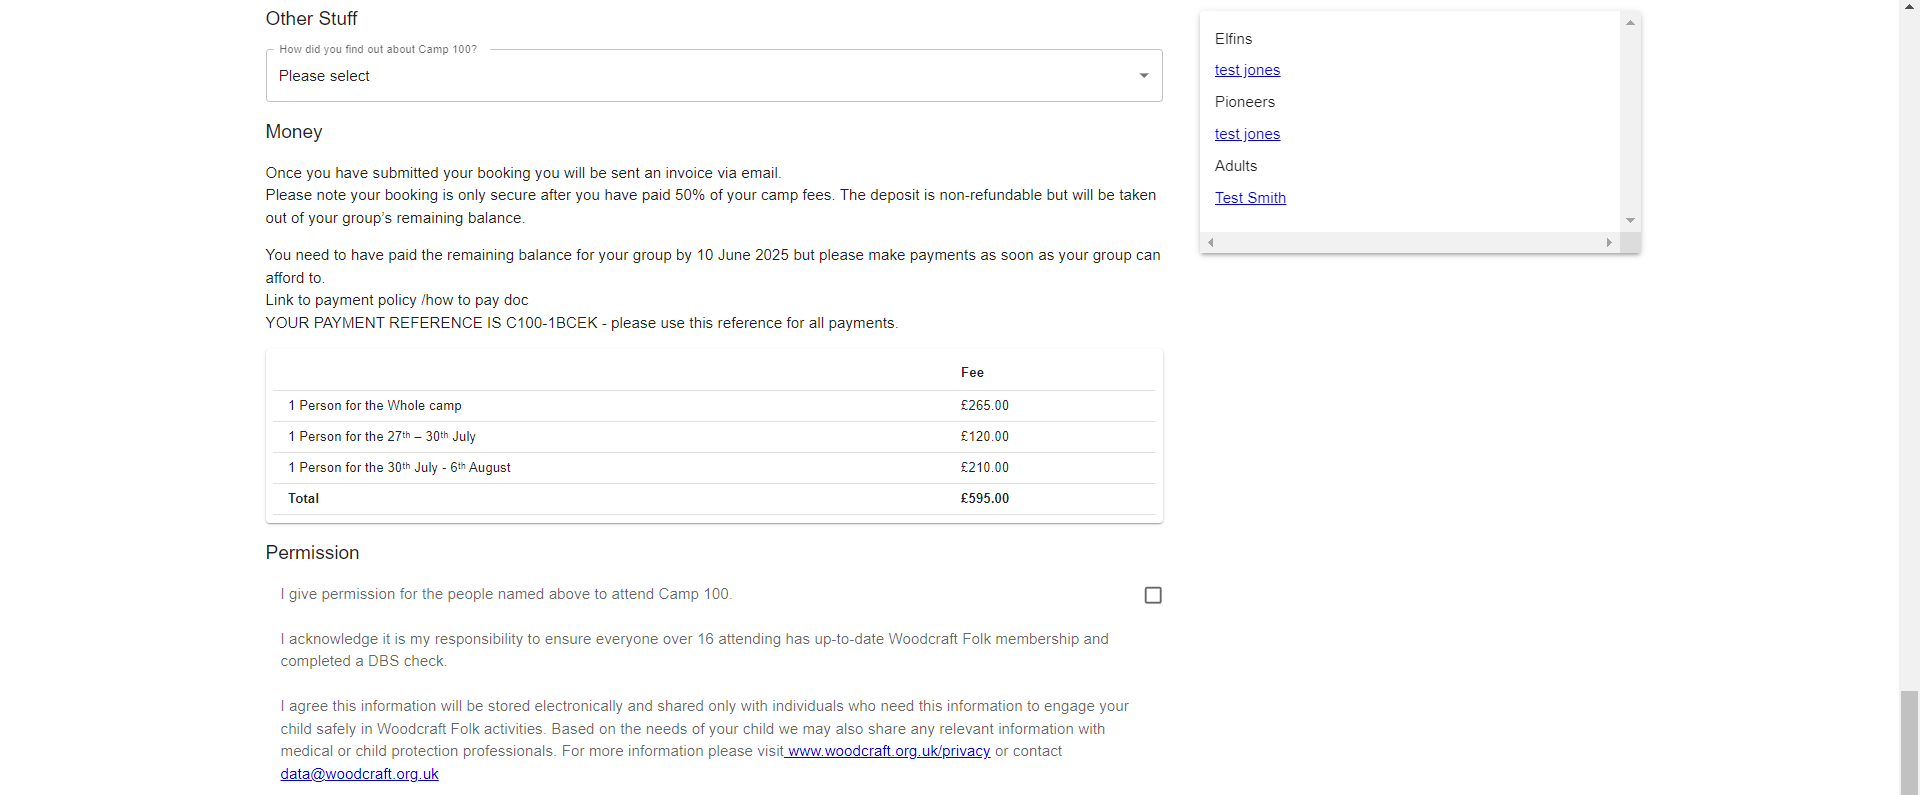
\includegraphics[width=0.9\textwidth]{assets/2-money.png}
        \caption{Section `Argent'}
    \end{figure}
    \item Continuez de descendre. Pour les r\'eservations individuelles, vous devez ajouter les informations d'une personne de plus de 16 ans en tant que contact d'urgence. Cela se fait dans la partie de contact d'urgence.
    \item Autorisez les personnes \`a participer et reconnaissez leur responsabilit\'e, puis envoyer la r\'eservation. Un \'ecran s'affiche pour confirmer les informations relatives au prix et donner un aperçu de la r\'eservation. Vous recevrez \'egalement un mail de confirmation avec une facture pour votre r\'eservation, qui sera modifi\'ee et renvoy\'ee chaque fois que vous modifierez votre r\'eservation. 
    \begin{figure}[H]
        \centering
        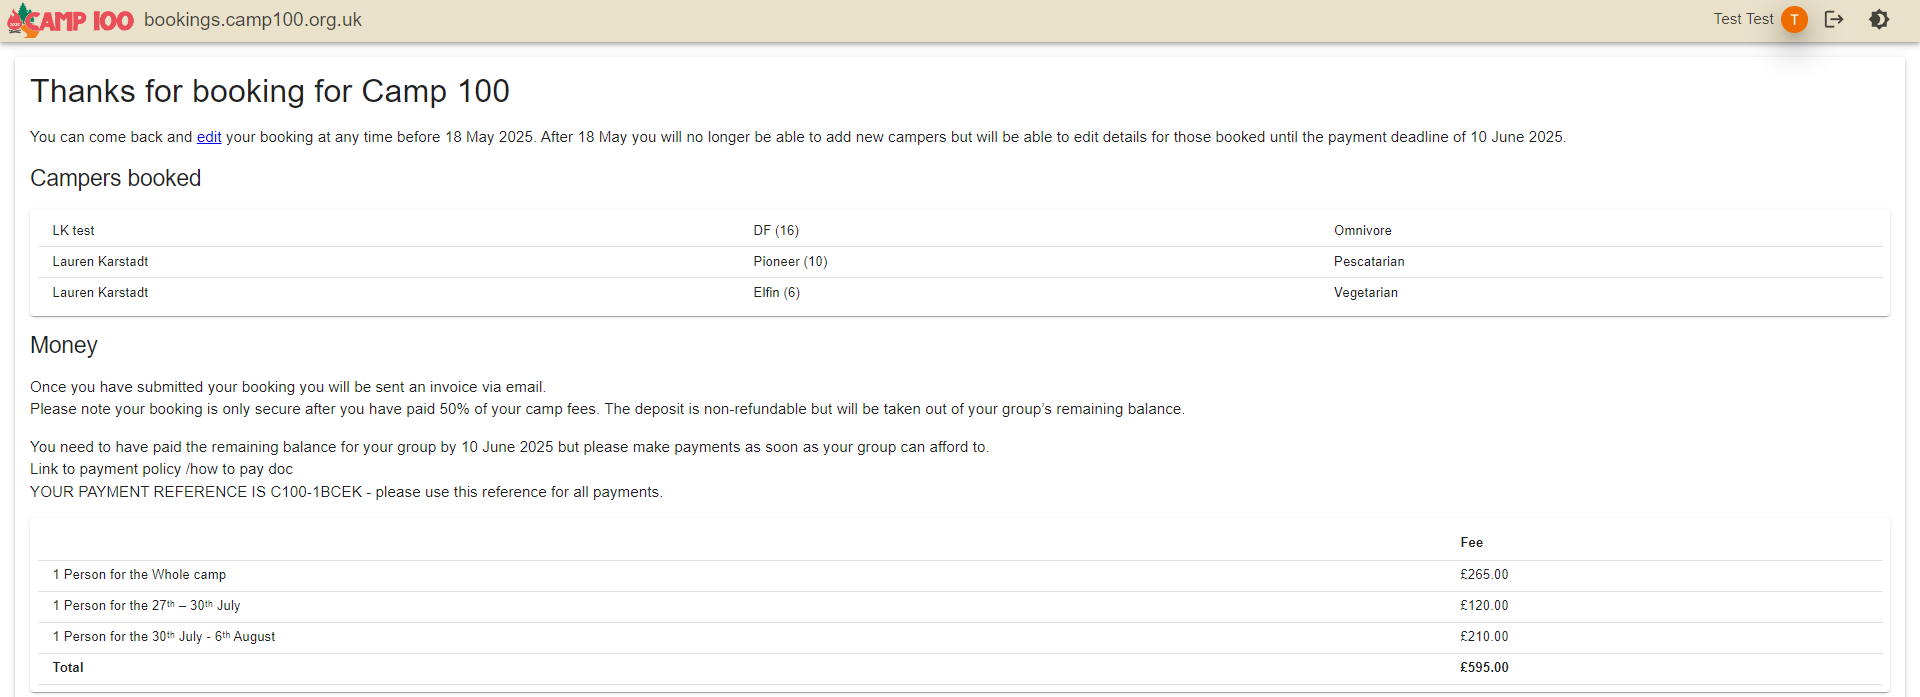
\includegraphics[width=0.9\textwidth]{assets/2-booking-confirmation.png}
        \caption{Page de confirmation de r\'eservation}
    \end{figure}
    
\end{enumerate}


\chapter[Etape 3: Modifier votre r\'eservation]{Etape 3: Modifier votre r\'eservation}
\label{chap:edit}

C'est compr\'ehensible que vous allez vouloir ajouter des informations ou des personnes \`a votre r\'eservation pour le Camp 100. 

Vous pouvez modifier votre r\'eservation \`a tout moment avant le 18 mai 2025. Apr\`es cette date vous ne pourrez plus ajouter de nouveaux campeurs, cependant vous pourrez toujours apporter des modifications \`a votre r\'eservation en cas de changement. Cependant, nous ne pouvons pas garantir d'apporter ces changements ou de vous rembourser. Le d\'elai jour pour le paiement du Camp 100 est le 10 juin 2025, apr\`es cette date vous devez vous rapprocher d'une membre de l'\'equipe de Woodcraft Folk pour modifier votre r\'eservation.
\begin{enumerate}
    \item Rendez vous sur \href{https://bookings.camp100.org.uk}{Camp 100 syst\`eme de r\'eservation}
    \item Connectez vous. Assurez vous d'utiliser le m\^eme service de connexion qu'avant, sinon vous devrez refaire une demande de r\'eservation. 
    \item Sur la page d'accueil vous trouverez un r\'ecapitulatif de votre r\'eservation et des informations de paiement.
    \item Cliquez sur `modifier ma r\'eservation'
    \item Vous allez \^etre redirig\'e vers la m\^eme page que pour faire votre r\'eservation et vous pourrez modifier votre r\'eservation dans le syst\`eme. Si vous utilisez la m\'ethode du tableau excel, vous pouvez mettre \`a jour votre tableau et ajouter/enlever/modifier les campeurs \`a tout moment avant la date limite. Assurez vous d'importer les informations dans le syst\`eme de r\'eservation afin que votre facture et vos informations de paiement soient mis \`a jour.
    \item Une fois que vous avez fini de modifier votre r\'eservation, vous devez rev\'erifier les permissions, puis cliquez sur envoyer la r\'eservation.
    \item Une fois que vous avez envoy\'e votre r\'eservation, un mail vous sera envoy\'e avec un r\'ecapitulatif des changements et une mise \`a jour de votre facture.
\end{enumerate}

\chapter{Paiement}
\label{chap:payment}

\begin{callout-orange}{Informations compl\'ementaires}
La politique de paiement et les informations compl\`etes sur la façon de payer peuvent \^etre trouv\'ees sur le \href{https://camp100.org.uk}{site Web du Camp 100}
\end{callout-orange}

Une fois que vous avez r\'eserv\'e, vous aurez une r\'ef\'erence de r\'eservation. Cette r\'ef\'erence aura comme format C100-XXXXX (les X seront remplac\'es par des num\'eros).
Cela permettra d'identifier votre r\'eservation. Vous devez l'utiliser au moment de payer afin que nous puissions bien identifier qui a fait le paiement et le d\'eduire de votre solde. 

\section{UK Payments}

Veuillez transf\'erer tous les paiements sur le compte suivant\\
\textbf{Nom du compte:} Woodcraft Folk\\
\textbf{Num\'ero de compte:} 2039 2756\\
\textbf{Code de tri:} 60 83 01

V\'erifiez votre r\'ef\'erence sur votre confirmation de r\'eservation, exemple : C100-XXXXX. Veuillez bien vous assurer d'utiliser cette r\'ef\'erence lors de vos paiements.

Si pour n'importe quelle raison, vous ne pouvez pas ajouter de r\'ef\'erence, veuillez envoyer un mail \`a info@camp100.org.uk pour nous informer du montant que vous avez transf\'er\'e, de la date du transfert et du nom de la personne qui a effectu\'e ce transfert. Nous pourrons ensuite faire le lien et mettre \`a jour votre solde.

\section{Paiements internationaux}

Veuillez transf\'erer tous les paiements vers ce compte:\\
\textbf{Code Swift (BIC):} NWBKGB2L\\
\textbf{Num\'ero IBAN:} GB93NWBK60023571418024\\
\textbf{Adresse de l'organisation:} \\
Holyoake House, Hanover Street, Manchester, M60 0AS, United Kingdom

V\'erifiez votre r\'ef\'erence sur votre confirmation de r\'eservation, exemple : C100-XXXXX. Veuillez bien vous assurer d'utiliser cette r\'ef\'erence lors de vos paiements.

Si pour n'importe quelle raison, vous ne pouvez pas ajouter de r\'ef\'erence, veuillez envoyer un mail \`a info@camp100.org.uk pour nous informer du montant que vous avez transf\'er\'e, de la date du transfert et du nom de la personne qui a effectu\'e ce transfert. Nous pourrons ensuite faire le lien et mettre \`a jour votre solde.


\chapter{Template Booking Form}
\label{chap:template-booking-form}

Un exemple du formulaire de r\'eservation a \'et\'e cr\'e\'e afin que les r\'ef\'erents puissent remplir toutes les informations de leur groupe avant de les rentrer dans le syst\`eme de r\'eservation. Certaines de ces informations sont uniquement pour des groupes et ne seront pas demand\'ees donc veuillez garder ces formulaires \`a titre informatif en cas d'urgence et d'informations m\'edicales. Le formulaire a \'et\'e inclus en dessous comme exemple, veuillez trouver une copie modifiable \href{https://drive.google.com/file/d/1oSFIkZQxzes3VTi5ZqPHCcAu4DiscvOm/view}{que vous pouvez t\'el\'echarge}. 

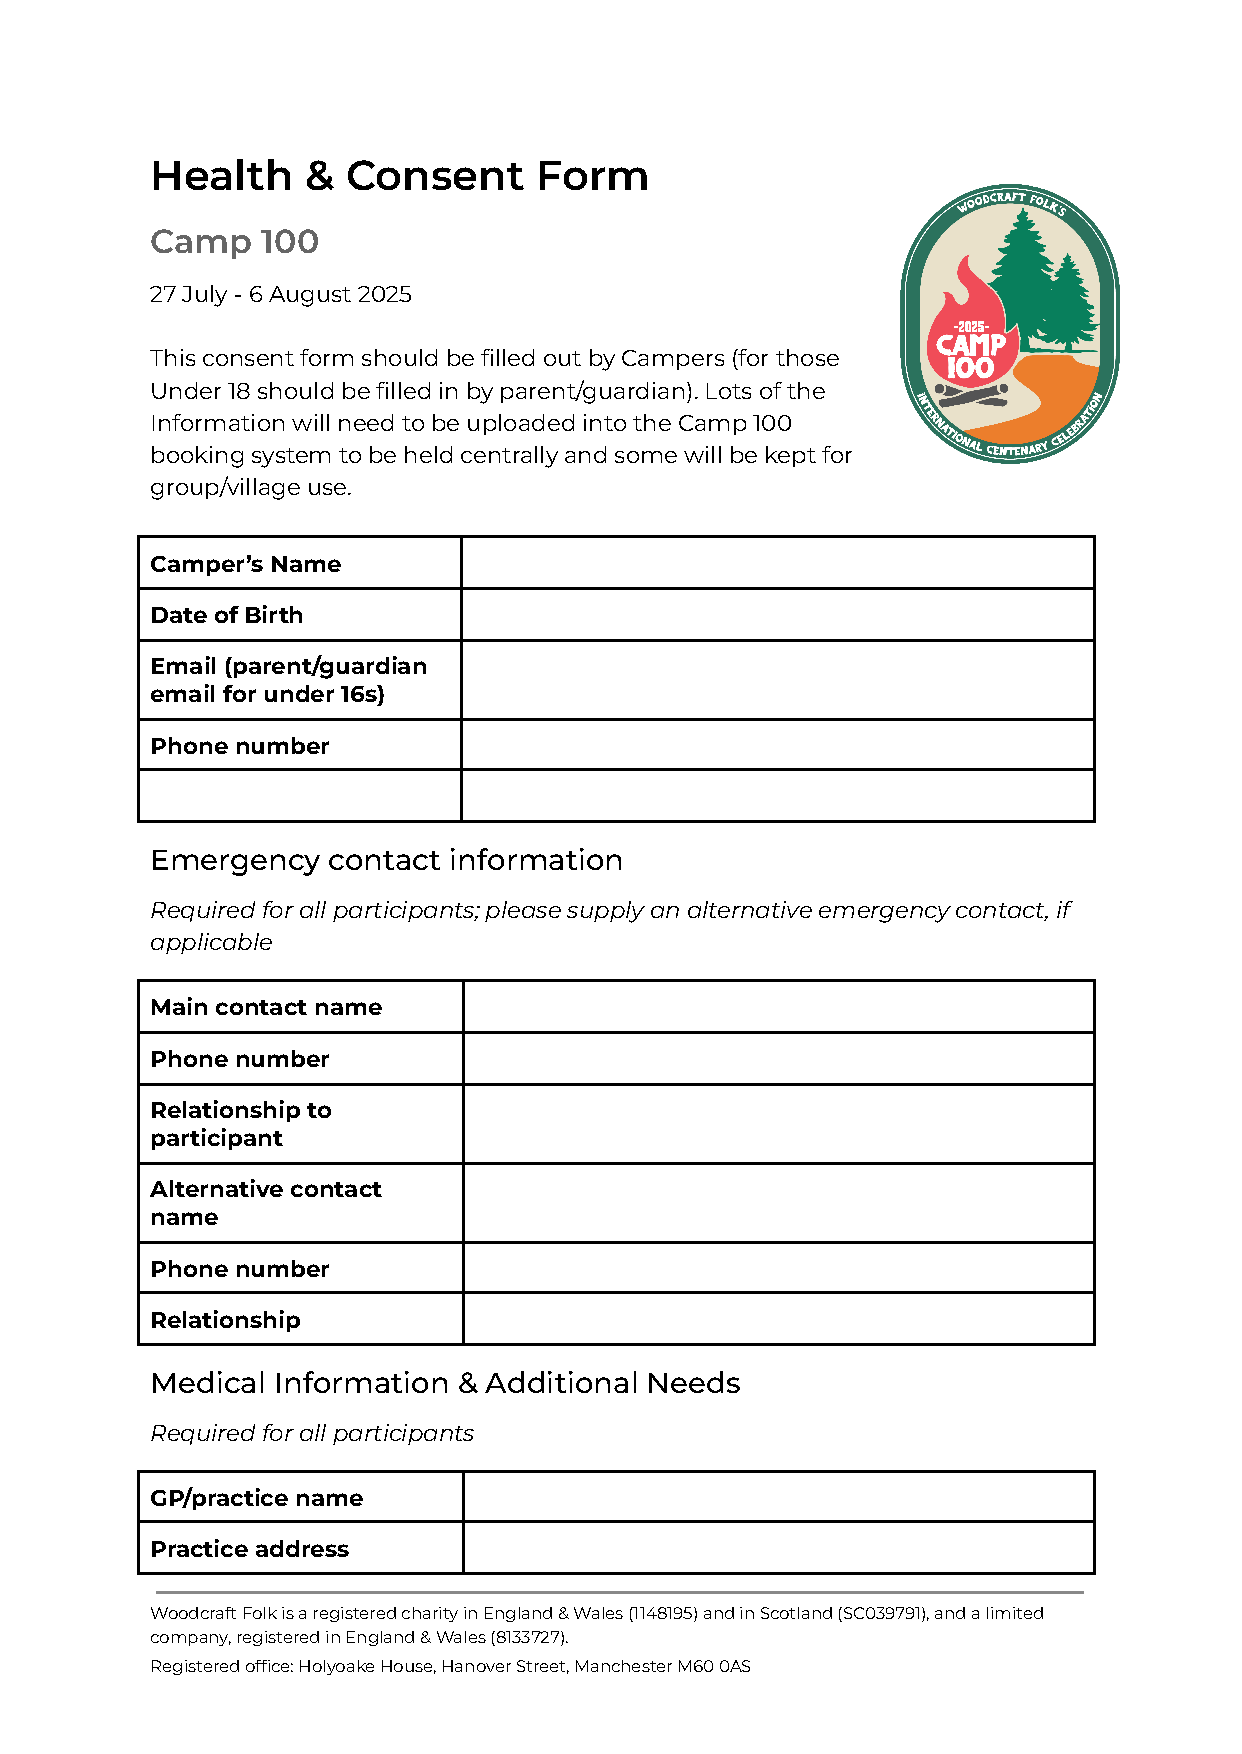
\includepdf[pagecommand={\pagestyle{fancy}}, scale=0.8, pages=-, frame]{assets/template-consent-form.pdf}

\makedocumentbackpage

\end{document}